\documentclass[12pt,a4paper,oneside]{article}
\usepackage[colorlinks=true, unicode]{hyperref}
\usepackage[utf8]{inputenc}
\usepackage[czech]{babel}
\usepackage{graphicx}
\usepackage{pdfpages}
\textwidth 16cm \textheight 25cm
\topmargin -1.3cm 
\oddsidemargin 0cm
\usepackage{footnote}
\pagestyle{empty}
\begin{document}
\title{Univerzální modul pro operační zesilovače}
\author{Jakub Kákona, kaklik@mlab.cz}
\maketitle

\thispagestyle{empty}
\begin{abstract}
Umožňuje zapojovat téměř všechna klasická zapojení operačních zesilovačů. 
\end{abstract}

\begin{figure} [htbp]
\begin{center}
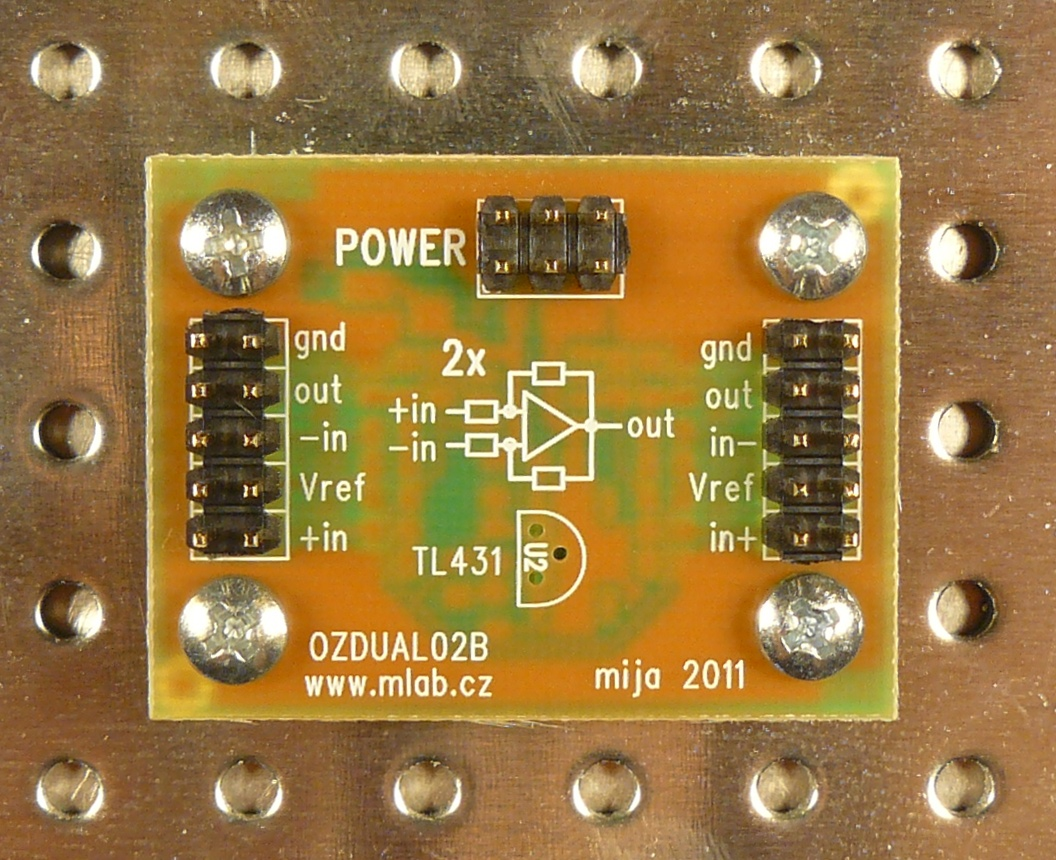
\includegraphics [width=100mm] {./img/OZDUAL02B_Top_Big.JPG} 
\end{center}
\end{figure}

\begin{figure} [b]

\includegraphics [width=25mm] {./img/OZDUAL02B_QRcode.png} 
\end{figure}

\newpage
\tableofcontents

\section{Technické parametry}
\begin{table}[htbp]
\begin{center}
\begin{tabular}{|c|c|p{4.7cm}|}
\hline
Parametr & Hodnota & Poznámka \\
\hline
Napájecí napětí POWER  & max 5V & \\ 
\hline
\end{tabular}
\end{center}
\end{table}

\section{Popis konstrukce}

\subsection{Zapojení}

Modul konstrukčně umožňuje realizaci všech standardních zapojení operačních zesilovačů využívajících asymetrického napájení.  Konkrétní volba zapojení je na znalostech konstruktéra.  Schéma modulu obsahuje pouze konstrukčně uvažované zapojení součástek. 

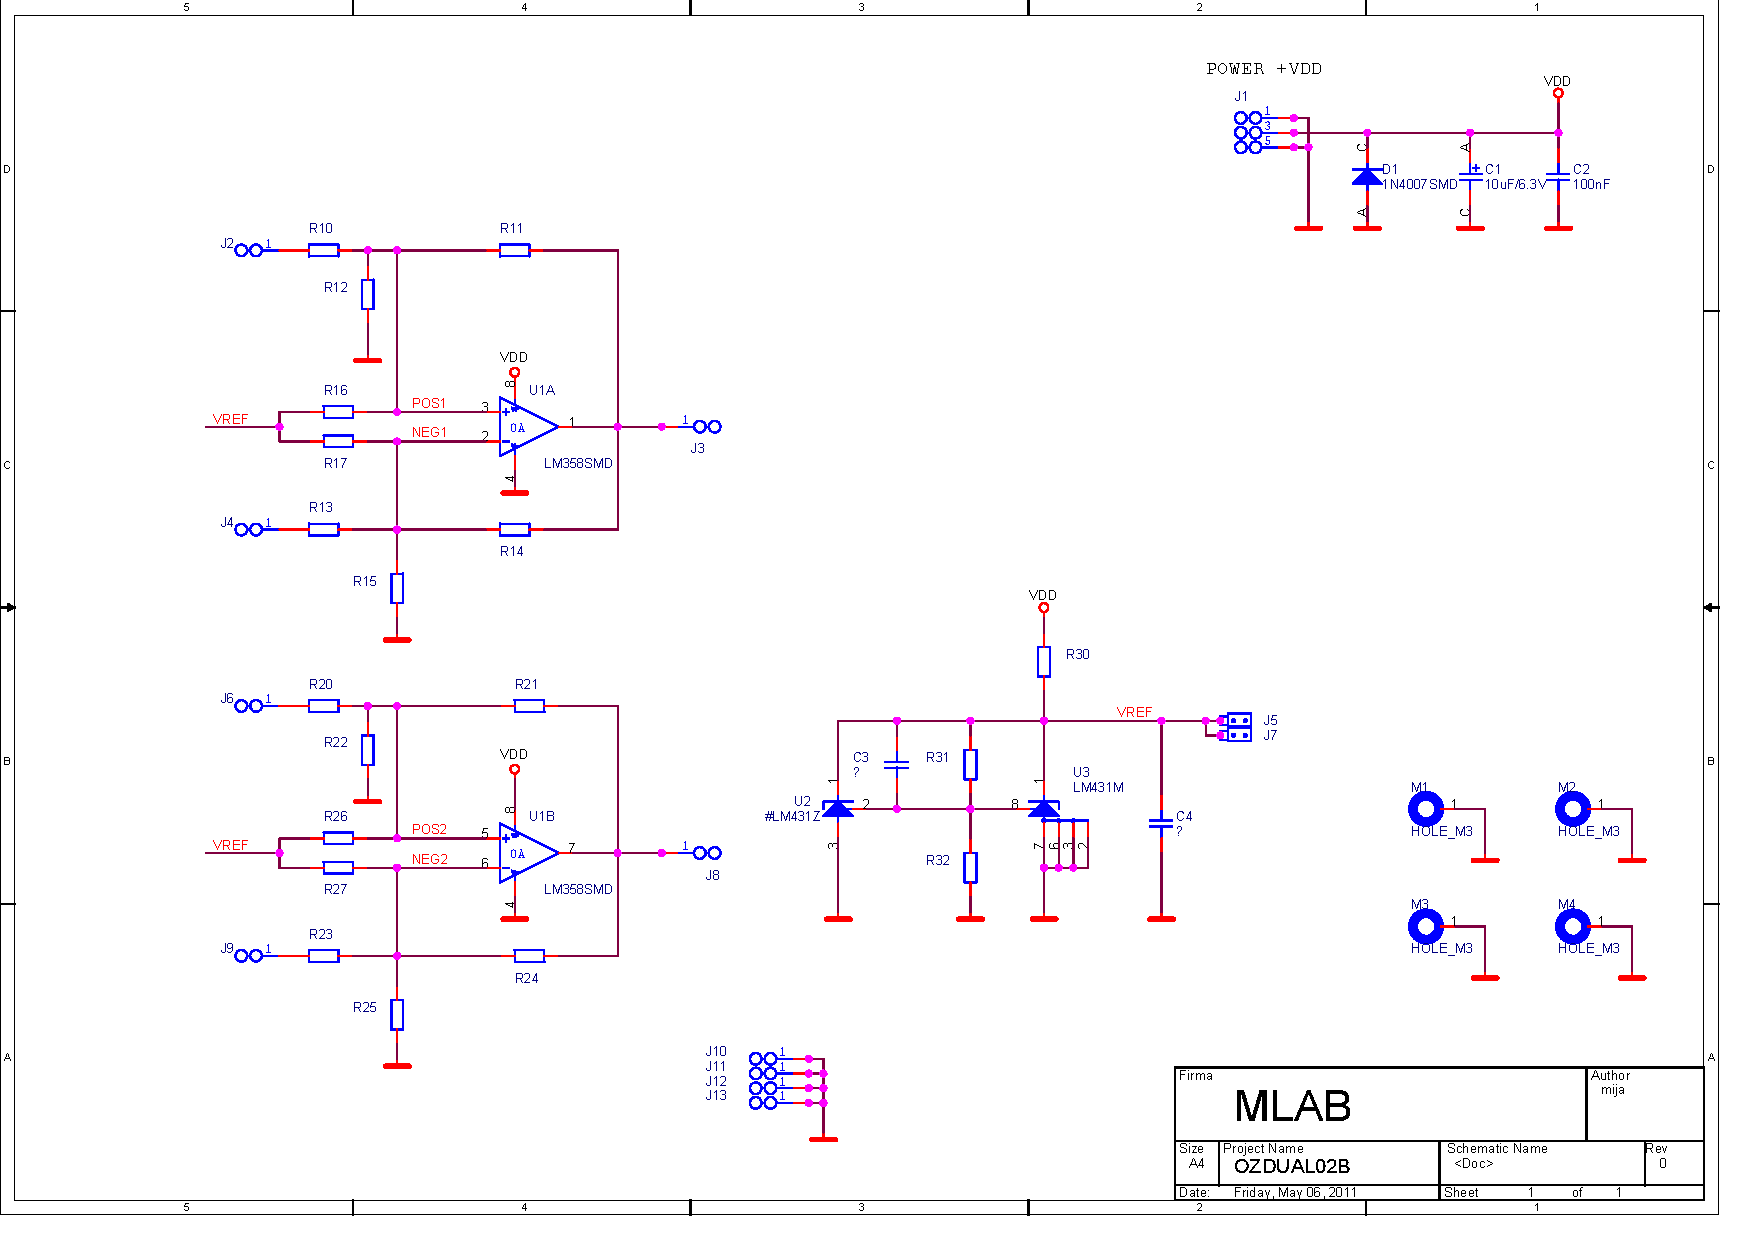
\includepdf[pages={1},landscape=true]{../../SCH/OZDUAL02B.pdf}

V zapojení modulu je obsažen lineární stabilizátor určený pro vytvoření referenčního napětí využitelného v zapojení. 

\subsection{Mechanická konstrukce}

Modul klasicky předpokládá uchycení na čtyřech šroubech, z důvodu lepšího EMC odstínění je vhodné zabezpečit aby všechny šrouby byly vodivě spojeny s podložkou.  

\section{Výroba a testování}

Plošný spoj je navržen jak pro ruční pájení, tak i pro osazování pomocí pasty.  Modul se testuje optickou kontrolou spojů a následným připojením na laboratorní zdroj s omezením proudu.

\subsubsection{Osazení}

Modul je možné osadit i ručně. Rozložení součástek je na Obr. \ref{fig:osazovaci_plan}. Pozice vyhrazené pro součástky v pouzdru 0805 lze použít i vícenásobně, což znamená, že například kondenzátory a rezistory lze letovat na sebe. Toto řešení usnadňuje realizaci kmitočtových filtrů a dalších zapojení kde jsou využity paralelní RC obvody. 

\begin{figure} [h!tbp]
  \centering
  %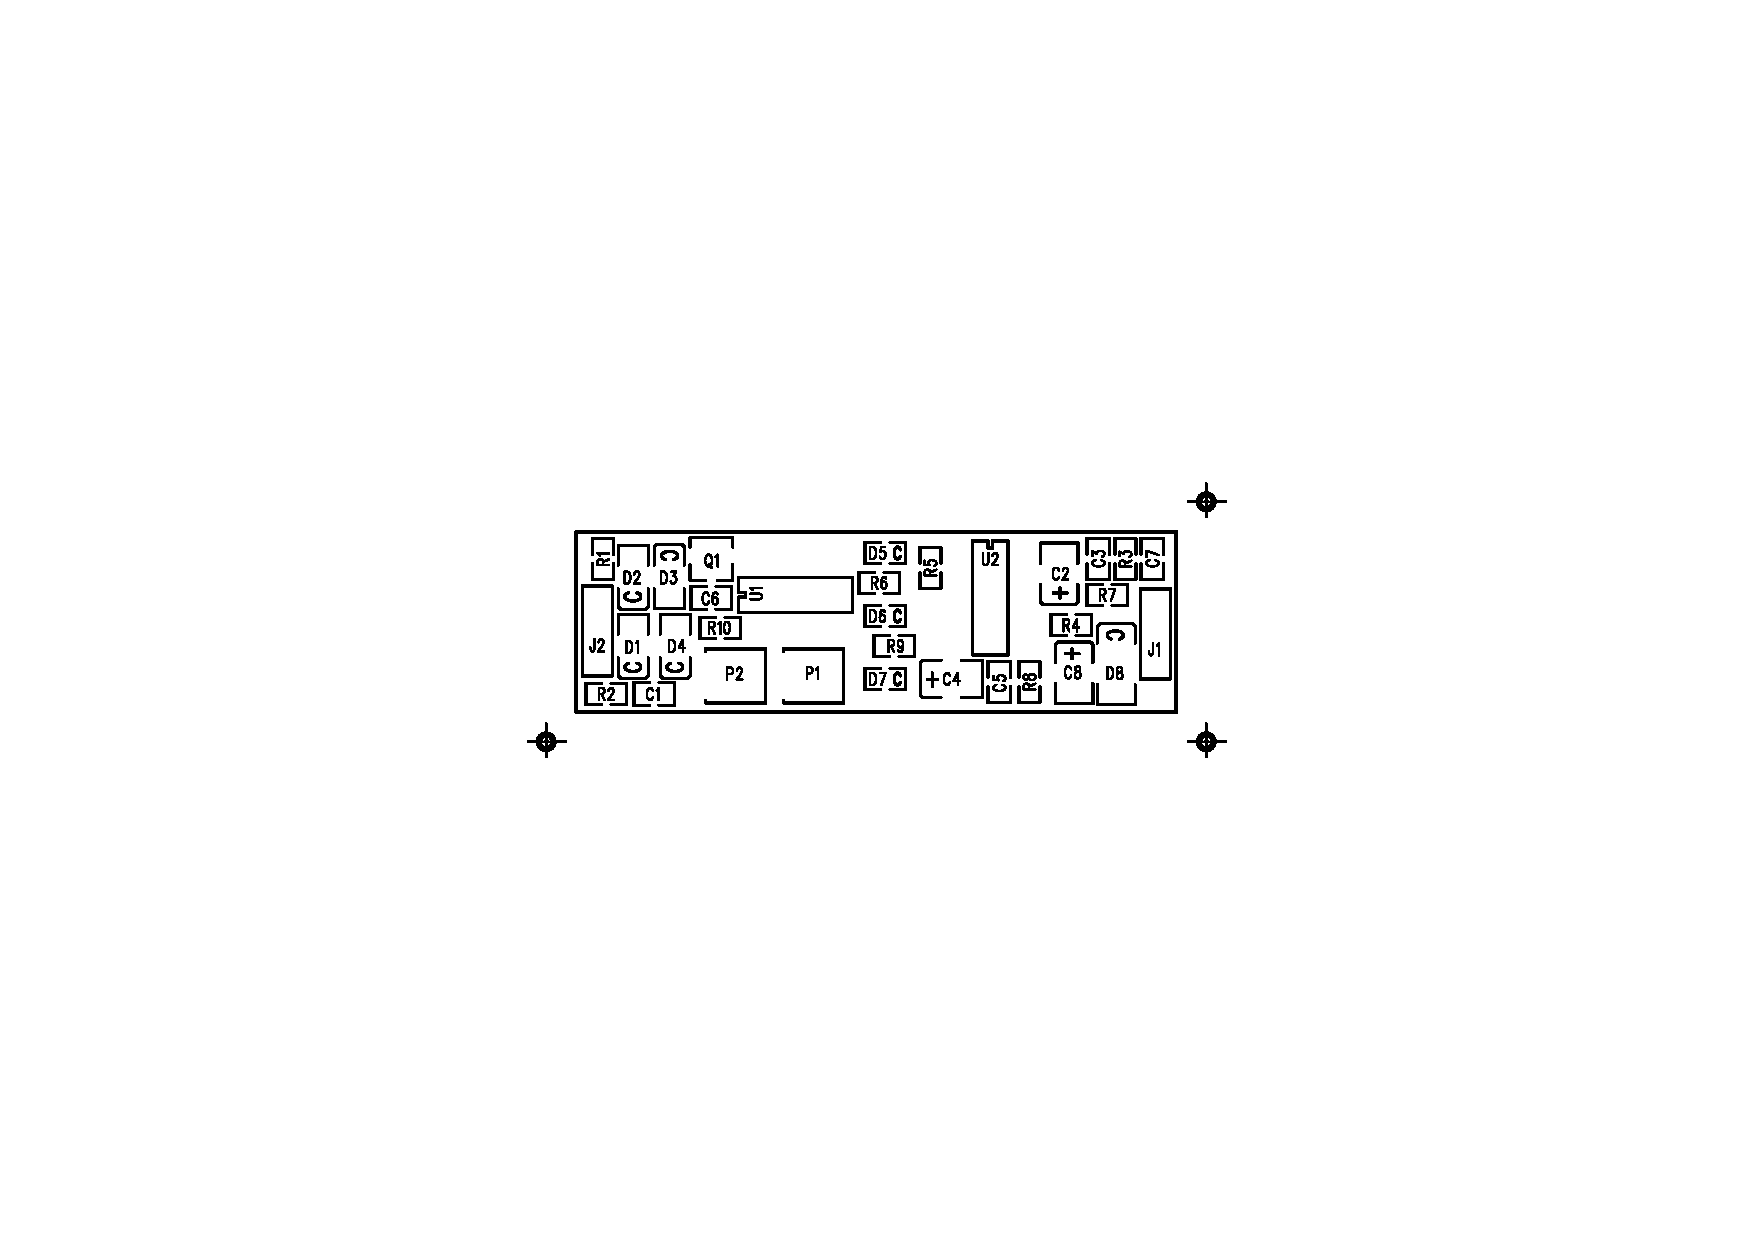
\includegraphics[trim = 7.5cm 12.5cm 7.5cm 12.5cm, clip, width=12cm]{../../CAM_DOC/O1.pdf}
  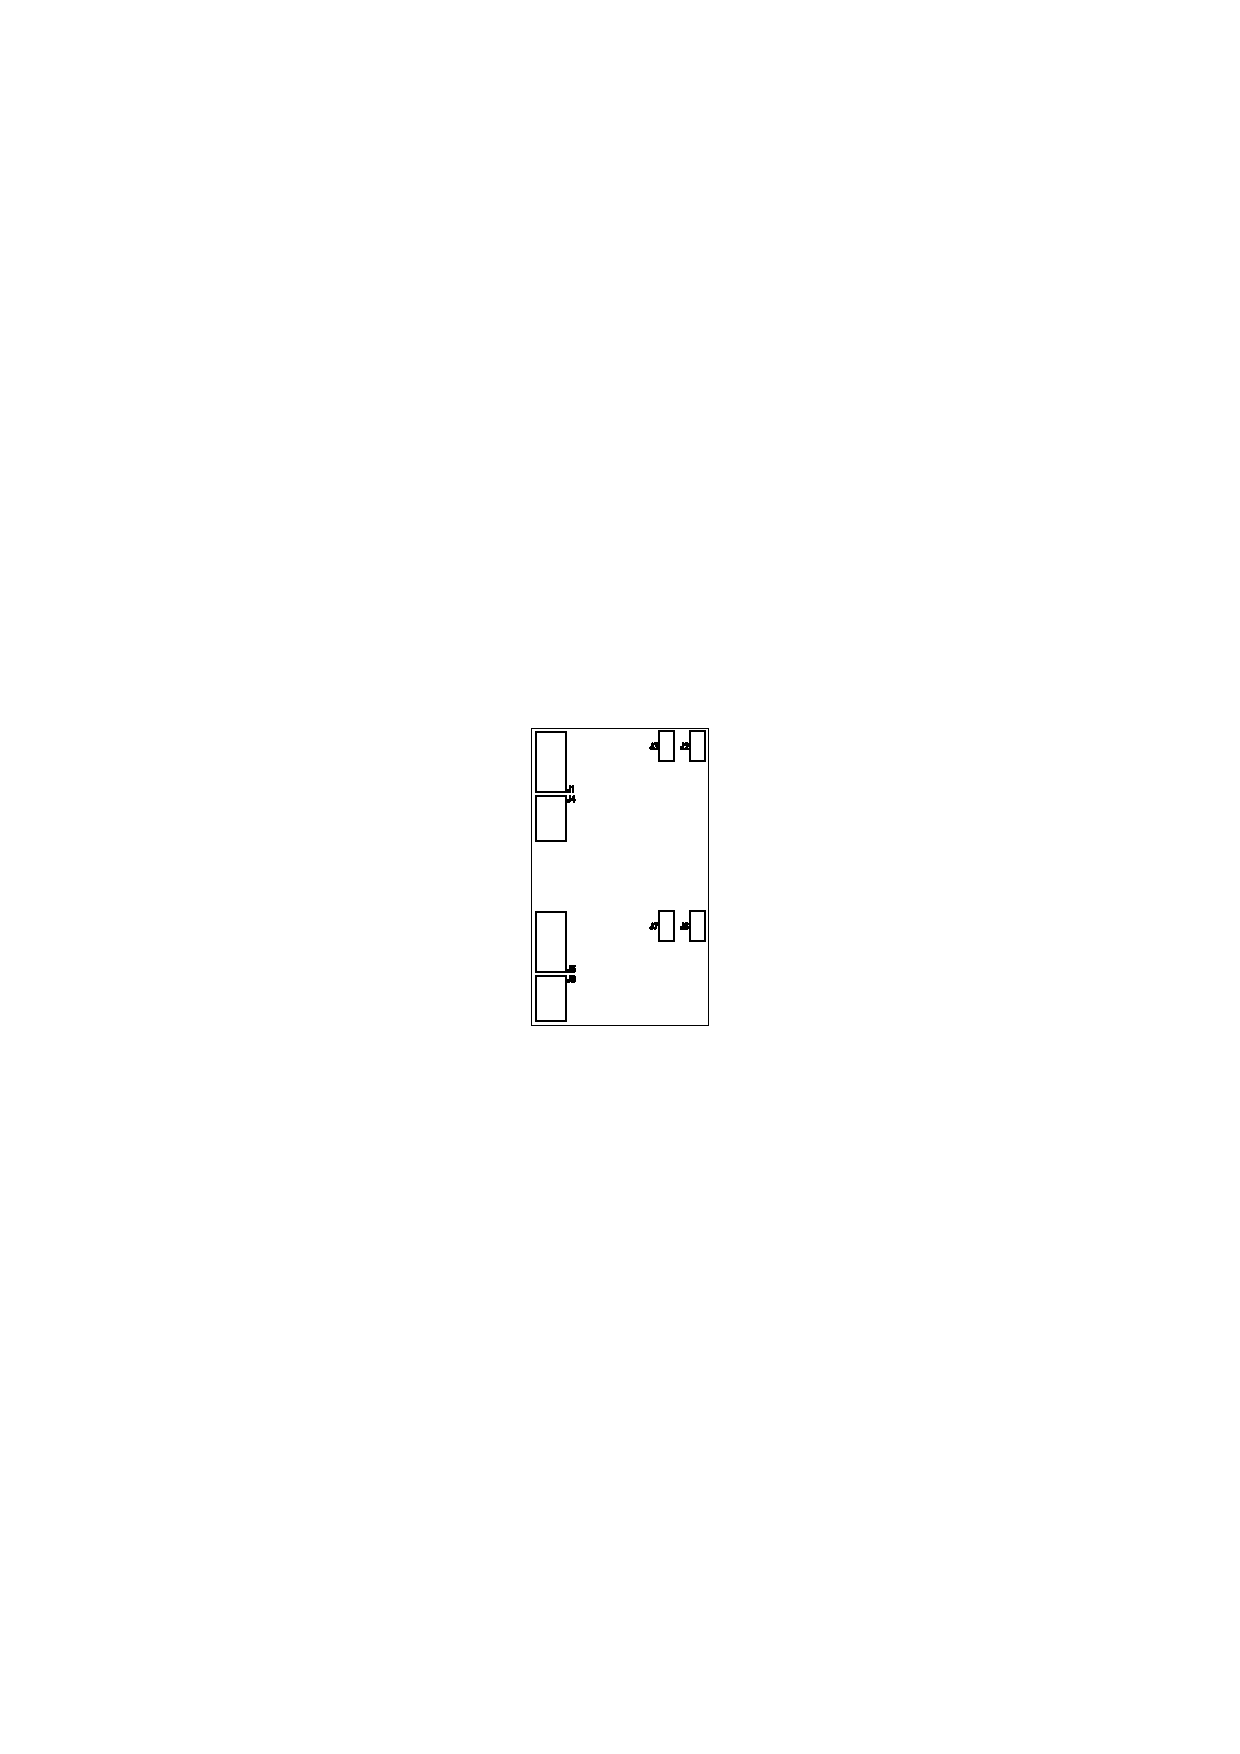
\includegraphics[trim = 6.0cm 11.5cm 6.0cm 11.5cm, clip, width=12cm]{../../CAM_DOC/O2.pdf}
  \caption{Osazovací plán horní a spodní strany plošného spoje}
  \label{fig:osazovaci_plan}
\end{figure}

Modul ze svého principu nemá předem definované hodnoty součástek v osazovacím plánu. Pro jeho použití doporučujeme pořízení celé řady rezitorů a kapacit v pouzdrech 0805 řazených v knize. 

\begin{thebibliography}{99}

\end{thebibliography}
\end{document}